%!TEX TS-program = xelatex
\documentclass[]{friggeri-cv}
\usepackage{afterpage}
\usepackage{hyperref}
\usepackage{color}
\usepackage{xcolor}
\usepackage{smartdiagram}
\usepackage{fontspec}
% if you want to add fontawesome package
% you need to compile the tex file with LuaLaTeX
% References:
%   http://texdoc.net/texmf-dist/doc/latex/fontawesome/fontawesome.pdf
%   https://www.ctan.org/tex-archive/fonts/fontawesome?lang=en
%\usepackage{fontawesome}
\usepackage{metalogo}
\usepackage{dtklogos}
\usepackage[utf8]{inputenc}
\usepackage{tikz}
\usetikzlibrary{mindmap,shadows}
\hypersetup{
    pdftitle={},
    pdfauthor={},
    pdfsubject={},
    pdfkeywords={},
    colorlinks=false,           % no lik border color
    allbordercolors=white       % white border color for all
}
\smartdiagramset{
    bubble center node font = \footnotesize,
    bubble node font = \footnotesize,
    % specifies the minimum size of the bubble center node
    bubble center node size = 0.5cm,
    %  specifies the minimum size of the bubbles
    bubble node size = 0.5cm,
    % specifies which is the distance among the bubble center node and the other bubbles
    distance center/other bubbles = 0.3cm,
    % sets the distance from the text to the border of the bubble center node
    distance text center bubble = 0.5cm,
    % set center bubble color
    bubble center node color = pblue,
    % define the list of colors usable in the diagram
    set color list = {lightgray, materialcyan, orange, green, materialorange, materialteal, materialamber, materialindigo, materialgreen, materiallime},
    % sets the opacity at which the bubbles are shown
    bubble fill opacity = 0.6,
    % sets the opacity at which the bubble text is shown
    bubble text opacity = 0.5,
}

\addbibresource{bibliography.bib}
\RequirePackage{xcolor}
\definecolor{pblue}{HTML}{0395DE}

\begin{document}
\header{Frans }{Ramirez Neyra}
      {Mechatronic Engineer}
      
% Fake text to add separator      
\fcolorbox{white}{gray}{\parbox{\dimexpr\textwidth-2\fboxsep-2\fboxrule}{%
.....
}}

% In the aside, each new line forces a line break
\begin{aside}
  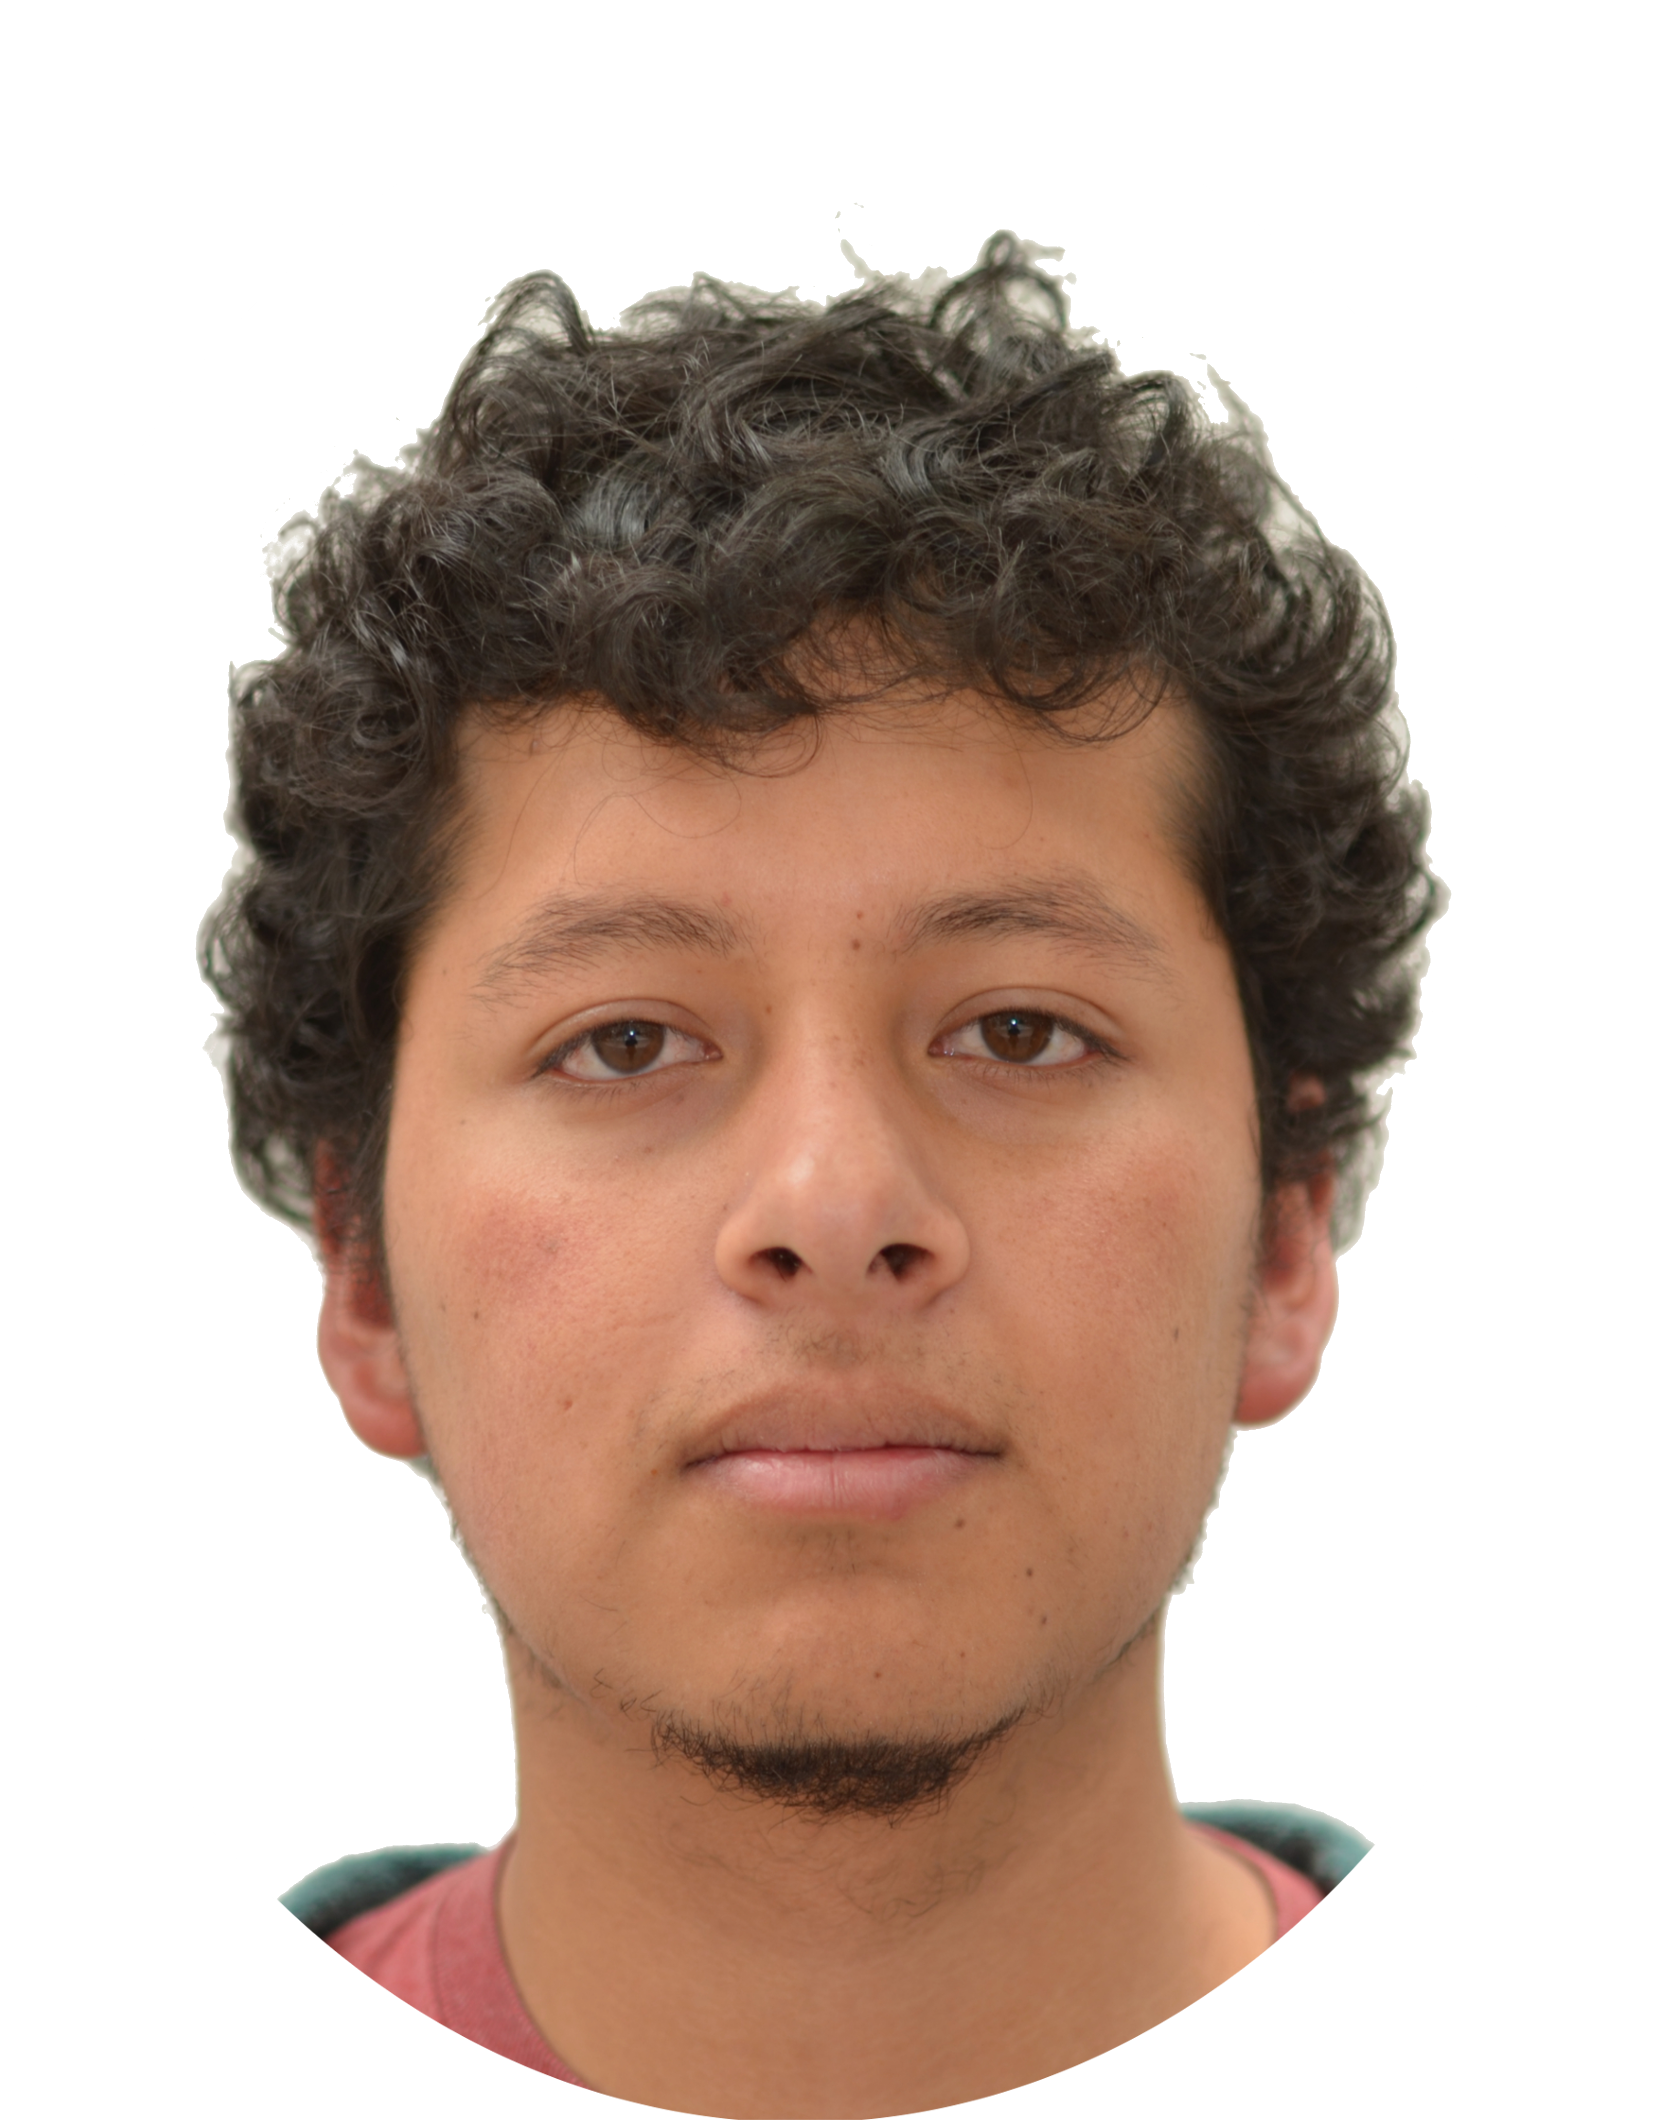
\includegraphics[scale=0.52]{img/Frans.png}
  \section{Address}
    Gutemberg 16
    Anzures, Mexico City
    ~
  \section{Tel \& Skype}
    +52 722 3632083
    frans.ramirez
    ~
  \section{Mail}
    \href{mailto:frans.caraveli@gmail.com}{\textbf{frans.caraveli@}\\gmail.com}
    ~
  \section{Web \& Git}
    \href{http://fransramirez.hol.es}{franscaraveli.hol.es}
    \href{https://github.com/Frans06}{github.com/Frans06}
    \href{https://repo.qbo.tech:5443/profile}{repo.qbo.tech/profile}
    \href{https://itesm.academia.edu/FransRamirezNeyra}{itesm.academia.edu/\\FransRamirezNeyra}
    ~
  % use  \hspace{} or \vspace{} to change bubble size, if needed
  \section{Programming}
    \smartdiagram[bubble diagram]{
        \textbf{Python},
        \textbf{Embbebing}\\\textbf{Sys},
        \textbf{ML}\\\textbf{TF/Keras}\\\textbf{Caffe\vspace{5mm}},
        \textbf{SQL}\\\textbf{NoSQL},
        \textbf{VHDL\vspace{3mm}},
        \textbf{MERN}\\\textbf{JS/React},
        \textbf{G O},
        \textbf{C/C++},
        \textbf{\hspace{2mm}Bash}
    }
    ~
  \section{Personal Skills}
    \smartdiagram[bubble diagram]{
        \textbf{Team}\\\textbf{Work},
        \textbf{Initiative},
        \textbf{Curiosity},
        \textbf{Problem}\\\textbf{Solving},
        \textbf{\vspace{2mm}Self Learner},
        \textbf{Stamina}
    }
    ~
\end{aside}
~
\section{Experience}
\begin{entrylist}
  \entry
    {03/17 - Now}
    {Software Engineer}
    {Connus International}
    {Company dedicated to the automation, integration and innovation of services and technologies oriented to the private security sector.\\\vspace{-3mm}
    \begin{itemize}
    \addtolength{\itemindent}{-4mm}
    	\item Integrate a LPR software solution trained by
ourselves of OpenALPR.\vspace{1mm}
    	\item Made the deployment of the new software to the border between
Mexico and the USA (in all the crossings).\vspace{1mm}
    	\item Development of an implementation of the AWS face recognition software as a solution for ATT in their communication towers.\vspace{1mm}
    	\item Development of a platform for IoT monitoring, which
integrates the face recognition, as well as infrastructure monitoring and sensor communication.\vspace{1mm}
		\item Improving prototypes to production development for a better performance and long time maintenance.\vspace{1mm}
		\item Improving to robust solutions implementing Debugging, Logging and Stress tests on Embbeded Systems.\vspace{1mm}
		\item Simple Implementation of ML technologies (Detectron, Fast-RCNN, YOLO) for simple Object Detection and data harvest.\vspace{1mm}
		\item Deploy of simple Docker implementation for Stacks and Swarm scaling On AWS.\vspace{1mm}
	\end{itemize}
    }
  \entry
    {06/18 - Now}
    {Manager \& Developer}
    {Nure\vspace{1mm}}
    {QBO Project - Reverse Image Search Engine Development based on a Modern Neuronal Network characteristics extraction. Then Vectorizing results and indexing them on Elastic Search to make searching easy and fast. I dockerize solution with nvidia runtime and docker orchestation for autoscaling.\\}
    \entry
    {05/10 - 09/16}
    {Research Intern}
    {McGill University\vspace{1mm}}
    {I help to Graduate and Postgraduate students on investigation projects\\\vspace{-3mm}
        \begin{itemize}
    		\addtolength{\itemindent}{-4mm}
    			\item Electronic and mechanical design of drones and control implementation.\vspace{1mm}
    			\item Automatic Maneuvers for Fixed Wings Airplanes research.\vspace{1mm}
    	\end{itemize}
    }
    \entry
    {09/16 - 12/16}
    {Project Investigator}
    {ITESM\vspace{1mm}}
    {Investigation in FPGA systems developing digital filters IIR or FIR and controllers. Contrasting and evaluating performance in analogic and digital filters and controllers}
\end{entrylist}
\\\vspace{-4mm}
\section{Education}
\begin{entrylist}
  \entry
    {2012 - 2016}
    {Bachelor's Degree in Mechatronic Engineering}
    {ITESM\vspace{1mm}}
    {Mechatronic Engineering oriented to Control and Electronics\\\vspace{-2mm}}
  \entry
    {2004, 2009}
    {Technical Degree in Informatics}
    {CEO Manuel T. Calle, Universidad San Luis Gonzaga\vspace{1mm}}
    {Wireless Connections and Internet Infrastructure\\}
\end{entrylist}

\newpage

\begin{aside}
~
~
~
  \section{OS Preference}
    \textbf{GNU/Linux}
\includegraphics[scale=0.40]{img/5stars.png}
    \textbf{MacOS}
\includegraphics[scale=0.40]{img/4stars.png}
    \textbf{Windows}
\includegraphics[scale=0.40]{img/2stars.png}
    ~
  \section{Places Lived}
    {Mexico, Peru, Canada}
    ~
  \section{Languages}
    \textbf{Spanish}
\includegraphics[scale=0.40]{img/5stars.png}
    \textbf{English}
\includegraphics[scale=0.40]{img/4stars.png}
    ~
\end{aside}

\section{Projects}
    \begin{itemize}
    \addtolength{\itemindent}{-4mm}    
      \item Design and construction of an scaled airplane, Aero Design SAE || Time: 6 month\vspace{1mm}
      \item Robot construction for FIRST Robotic Competition || Time: 3 Years\vspace{1mm}
      \item Development of a line following by camera car for FreeScale Cup || Time: 2 Years\vspace{1mm}
      \item Investigation in XO computer complement development. || Time: 1 Year\vspace{1mm}

    \end{itemize}
\section{Honors \& Awards}
\begin{entrylist}
  \entry
    {12/2016}
    {Doble Golden Lamb Award}
    {Career Activities}
    {Awarded by take part of several activities along the Career }
  \entry
    {12/2016}
    {Excelence Honorific Mention }
    {Best GPA on Career Generation}
    {Awarded by having the best GPA up to 9.5 out of 10}
\end{entrylist}

\end{document}
